\documentclass[letterpaper,10pt,conference]{ieeeconf}
\IEEEoverridecommandlockouts
\overrideIEEEmargins
\usepackage[T1]{fontenc}
\renewcommand{\sfdefault}{ptm}
\renewcommand{\ttdefault}{ptm}
\usepackage{dblfloatfix}
\usepackage[nospread]{flushend}
\usepackage{amsmath,amssymb,bm,graphicx,booktabs,array,tabularx,cite,tikz,capt-of}
\usepackage[hidelinks]{hyperref}
\urlstyle{rm}
\SetMathAlphabet{\mathsf}{normal}{OT1}{ptm}{m}{n}
\SetMathAlphabet{\mathsf}{bold}{OT1}{ptm}{b}{n}
\hypersetup{pdftitle={LAB4: Polynomial Trajectory Optimization and Unity Flight Evaluation},pdfauthor={Shuyu Li}}
\renewcommand{\topfraction}{0.96}
\renewcommand{\dbltopfraction}{0.96}
\renewcommand{\bottomfraction}{0.90}
\renewcommand{\textfraction}{0.04}
\renewcommand{\floatpagefraction}{0.80}
\renewcommand{\dblfloatpagefraction}{0.80}
\setlength{\textfloatsep}{9pt plus 2pt minus 2pt}
\setlength{\dbltextfloatsep}{9pt plus 2pt minus 2pt}
\setlength{\floatsep}{7pt plus 1pt minus 1pt}
\setlength{\dblfloatsep}{7pt plus 1pt minus 1pt}
\setlength{\intextsep}{8pt plus 1pt minus 1pt}
\setlength{\abovecaptionskip}{5pt}
\setlength{\belowcaptionskip}{2pt}
\setcounter{topnumber}{4}
\setcounter{bottomnumber}{3}
\setcounter{totalnumber}{6}
\setcounter{dbltopnumber}{3}
\makeatletter
\setlength{\@fptop}{0pt}
\setlength{\@dblfptop}{0pt}
\setlength{\@fpsep}{9pt}
\setlength{\@dblfpsep}{9pt}
\makeatother
\usetikzlibrary{arrows.meta,positioning}
\definecolor{teal}{HTML}{0000FF}
\definecolor{navy}{HTML}{000000}
\definecolor{pale}{HTML}{FFFFFF}
\newcolumntype{Y}{>{\raggedright\arraybackslash}X}
\newcommand{\dd}{\mathrm d}
\newcommand{\norm}[1]{\lVert#1\rVert}
\newcommand{\R}{\mathbb R}
\newcommand{\figone}[3]{\begin{figure}[!tbp]\centering\includegraphics[width=\columnwidth]{figures/#1.pdf}\caption{#2}\label{#3}\end{figure}}
\newcommand{\figwide}[3]{\begin{figure*}[!tbp]\centering\includegraphics[width=\textwidth]{figures/#1.pdf}\caption{#2}\label{#3}\end{figure*}}
\title{\LARGE\bf LAB4: Polynomial Trajectory Optimization and Unity Flight Evaluation for Drone Racing}
\author{Shuyu Li\thanks{Robot Integration Project course. Student ID: 24020036035. Laboratory report, November 9, 2026.}}
\IEEEaftertitletext{%
\begin{minipage}{\textwidth}\centering
\begin{tikzpicture}[box/.style={draw=black,fill=white,line width=0.7pt,text width=27mm,inner sep=1.1mm,minimum height=29mm,align=center,font=\rmfamily\scriptsize},>=Stealth,node distance=6mm]
\node[box](a){{\bfseries Course geometry}\\[3pt]
\raisebox{0pt}[9mm][0mm]{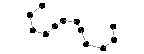
\includegraphics[width=24mm,height=9mm,keepaspectratio]{figures/pipeline_geometry.pdf}}\\[3pt]Gate centres $\bm g_i$\\Gate headings $\psi_i$\\Endpoint states};
\node[box,line width=1pt,right=of a](b){{\bfseries\color{blue} Trajectory planning}\\[3pt]
\raisebox{0pt}[9mm][0mm]{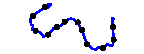
\includegraphics[width=24mm,height=9mm,keepaspectratio]{figures/pipeline_reference.pdf}}\\[3pt]Minimum snap /\\rigid-body planning\\Timing and constraints};
\node[box,right=of b](c){{\bfseries Reference sampling}\\[3pt]
\raisebox{0pt}[9mm][0mm]{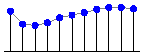
\includegraphics[width=24mm,height=9mm,keepaspectratio]{figures/pipeline_samples.pdf}}\\[3pt]$\bm p_d,\bm v_d,\bm a_d$\\$R_d,\bm\omega_d$\\20 ms team grid};
\node[box,right=of c](d){{\bfseries Feedback control}\\[3pt]
\raisebox{0pt}[9mm][0mm]{\begin{tikzpicture}[x=8mm,y=8mm,line width=.55pt,>=Stealth]
\draw(.25,.55)circle(.12);\draw(.18,.55)--(.32,.55);\draw(.25,.48)--(.25,.62);
\draw(.8,.32)rectangle(1.3,.78);
\node[draw=none,text width=3mm,minimum height=2mm,minimum width=3mm,inner sep=0pt,font=\rmfamily\tiny]at(1.05,.55){$K$};
\draw[->](-.1,.55)--(.13,.55);\draw[->](.37,.55)--(.8,.55);\draw[->](1.3,.55)--(2,.55);
\draw[->](1.7,.55)--(1.7,0)-|(.25,.43);
\draw(.07,.26)--(.19,.26);
\end{tikzpicture}}\\[3pt]Feedforward + feedback\\Rotor allocation\\$\Omega_1,\ldots,\Omega_4$};
\node[box,right=of d](e){{\bfseries Unity dynamics}\\[3pt]
\raisebox{0pt}[9mm][0mm]{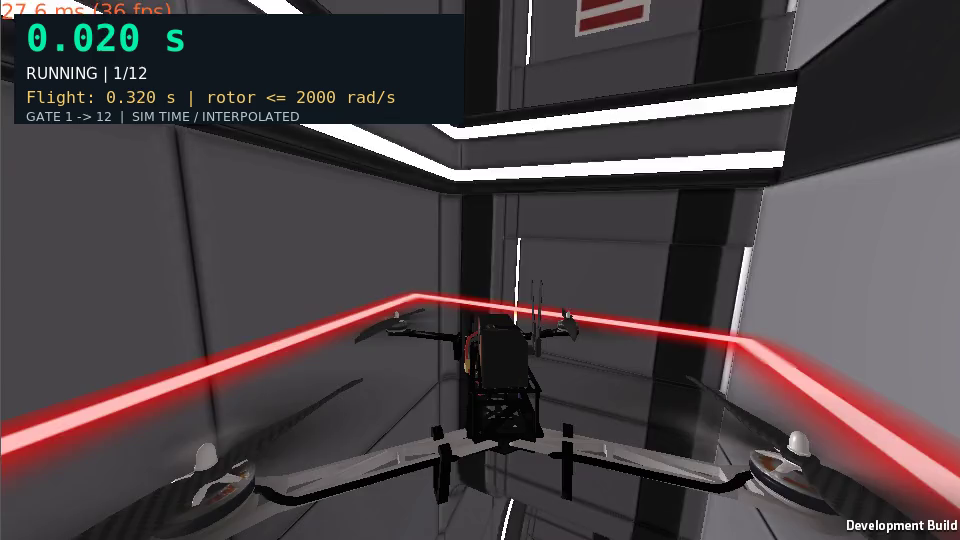
\includegraphics[width=24mm,height=9mm,keepaspectratio]{figures/unity_preview.png}}\\[3pt]
Native physics\\$\bm p,\bm v,R,\bm\omega$\\Gate passage};
\draw[->,line width=0.7pt](a)--(b);\draw[->,line width=0.7pt](b)--(c);
\draw[->,line width=0.7pt](c)--(d);\draw[->,line width=0.7pt](d)--(e);
\node[box,text width=91mm,minimum height=17mm,below=7mm of b,xshift=18mm](f){{\bfseries Measured Unity race}\\[3pt]
\setlength{\tabcolsep}{5mm}\begin{tabular}{ccc}
{\large\bfseries\color{blue} 0.640 s}&{\large\bfseries 12/12}&{\large\bfseries 0.06267 m}\\[2pt]
Gate 1--12, sim. time&Ordered gates&Timed RMSE
\end{tabular}};
\draw[->,line width=0.7pt](c.south)--++(0,-5mm)-|(f.north);
\draw[->,line width=0.7pt](e.east)--++(5mm,0)|-(f.east);
\draw[->,dashed,line width=0.7pt](e.south)--++(0,-7mm)-|node[pos=.25,below,font=\rmfamily\scriptsize]{measured state}(d.south);
\end{tikzpicture}
\captionof{figure}{Planning, execution, and measured Unity performance. The small graphics show the course geometry, stored racing reference, and sampled reference states. Native state closes the control loop and supplies gate-passage, timing, and tracking measurements.}
\label{fig:pipeline}
\end{minipage}\vspace{4pt}}
\begin{document}
\maketitle
\thispagestyle{empty}\pagestyle{empty}
\begin{abstract}
Fast drone flight requires a reference that the controller can track through each gate.
We solve the single- and multi-segment optimization problems in MIT VNAV LAB4, then evaluate tracking in individual numerical experiments and a team Unity flight.
Exact solutions describe how polynomial degree affects cost, and a variational derivation gives the minimum-snap boundary conditions.
On a six-segment numerical course, optimizing internal waypoint derivatives reduces snap cost by 98.98\% at the same 12 s duration compared with stopping at every waypoint.
Matched experiments isolate acceleration lag and saturation.
In Unity, a discrete rigid-body reference and synchronous feedback controller traverse all twelve gates in 0.640 s of simulation time, measured from gate 1 to gate 12.
Timed position RMSE is 0.06267 m, and the minimum point-to-aperture-edge margin is 0.287 m.
No collision is recorded during racing or braking.
Thirteen saved valid runs round to the same 0.640 s score.
The numerical experiments quantify timing-dependent tracking error, and the Unity run measures gate passage under the stated simulator settings.
\end{abstract}
\section{Introduction}
A racing trajectory specifies a path and the time spent along it.
Waypoint positions determine where the drone must pass, while trajectory derivatives determine the controller's motion commands.
Shortening traversal time can increase tracking error even when the spatial curve stays unchanged.

The LAB4 exercises\cite{mit} cover single-segment optimization, multi-segment minimum-snap planning, and desired-state generation for racing.
We solve the requested quadratic programs and distinguish continuity constraints from optimality conditions.
Numerical experiments compare two waypoint treatments at equal duration, then vary duration with the spatial path and controller fixed.
The VNAV2021 nodes\cite{code} provide the course implementation.

The individual experiments examine when higher polynomial degree reduces cost, how intermediate stops affect smoothness, and how time compression changes acceleration demand and position error.
Matched ablations isolate lag and saturation, and a response-time sweep tests duration selection across different lags.
The team experiment applies a rigid-body reference and synchronous controller to the twelve-gate Unity course.
Sections~II--VI contain the individual analysis and experiments; Section~VII reports the team flight.
\section{Individual Deliverable 1: Single-Segment Optimization}
\subsection{Position Constraints and a Global Lower Bound}
Consider the scalar, normalized-time problem
\begin{equation}
\min_P J=\int_0^1\dot P(t)^2\dd t,\quad P(0)=0,\quad P(1)=1.\label{eq:single}
\end{equation}
For a linear polynomial $P(t)=p_1t$, the terminal position gives $p_1=1$, so $P^*(t)=t$ and $J^*=1$.
This solution achieves a lower bound that applies to every feasible polynomial:
\begin{equation}
\int_0^1\dot P^2\dd t\geq\left(\int_0^1\dot P\dd t\right)^2=1.
\end{equation}
Equality in the Cauchy--Schwarz inequality requires constant velocity.
Constant-speed motion therefore attains the minimum cost at every polynomial degree that admits it.
\subsection{Quadratic-Program Formulation}
Let $P(t)=\sum_{i=1}^Np_it^i$ and $\bm p=[p_1,\ldots,p_N]^\mathsf T$.
The constant coefficient is zero because $P(0)=0$.
Direct integration gives
\begin{equation}
J=\bm p^\mathsf TQ\bm p,\qquad Q_{ij}=\frac{ij}{i+j-1},\quad i,j=1,\ldots,N.
\end{equation}
For degree two, the objective and endpoint constraint are
\begin{equation}
Q_2=\begin{bmatrix}1&1\\1&4/3\end{bmatrix},\quad
A_2=\begin{bmatrix}1&1\end{bmatrix},\quad b=1.
\end{equation}
Substituting $p_1=1-p_2$ yields $J=1+p_2^2/3$, whose minimum is attained at $(p_1,p_2)=(1,0)$.
For degree three,
\begin{equation}
Q_3=\begin{bmatrix}1&1&1\\1&4/3&3/2\\1&3/2&9/5\end{bmatrix},\quad
A_3=\begin{bmatrix}1&1&1\end{bmatrix}.
\end{equation}
The minimizer is $(1,0,0)^\mathsf T$, again with cost one.
A solver using the objective $\frac12\bm p^\mathsf TH\bm p$ therefore requires $H=2Q$.
The two objective conventions give the same minimizer.
\subsection{An Additional Terminal-Velocity Constraint}
Next impose $\dot P(1)=-2$.
For a quadratic polynomial,
\begin{equation}
\begin{bmatrix}1&1\\1&2\end{bmatrix}\begin{bmatrix}p_1\\p_2\end{bmatrix}
=\begin{bmatrix}1\\-2\end{bmatrix}.
\end{equation}
Both coefficients are fixed, giving
\begin{equation}
P_2^*(t)=4t-3t^2,\qquad J_2^*=4.
\end{equation}
For a cubic polynomial, the constraint matrix is
\begin{equation}
A=\begin{bmatrix}1&1&1\\1&2&3\end{bmatrix},\qquad
\bm b=\begin{bmatrix}1\\-2\end{bmatrix}.
\end{equation}
The constraints imply $p_1=4+p_3$ and $p_2=-3-2p_3$.
Substitution into the objective gives
\begin{align}
J&=4+p_3+\frac{2}{15}p_3^2\\
&=\frac{17}{8}+\frac{2}{15}\left(p_3+\frac{15}{4}\right)^2.
\end{align}
Consequently,
\begin{equation}
\boxed{P_3^*(t)=\frac14t+\frac92t^2-\frac{15}{4}t^3,\quad J_3^*=\frac{17}{8}.}
\end{equation}
The cubic polynomial lowers the cost by 46.875\%.
Its additional degree of freedom redistributes velocity while satisfying both endpoint positions and the terminal-velocity constraint.
Both constrained solutions overshoot the terminal position and return with negative velocity (Fig.~\ref{fig:single}).
\figone{icra_single}{Exact position and velocity profiles for the single-segment problems. The blue curve is optimal for the position-only problem at degrees one through three. Adding $\dot P(1)=-2$ gives the quadratic and cubic profiles shown. The cubic profile redistributes velocity and reduces cost from 4 to 2.125.}{fig:single}
\begin{table}[t]\centering
\caption{Exact solutions of the single-segment exercises.}
\label{tab:single}\small
\begin{tabular}{lclc}\toprule
Constraints&Degree&Coefficients $(p_1,p_2,p_3)$&$J^*$\\\midrule
Position only&1&$(1)$&1\\
Position only&2&$(1,0)$&1\\
Position only&3&$(1,0,0)$&1\\
Also $\dot P(1)=-2$&2&$(4,-3)$&4\\
Also $\dot P(1)=-2$&3&$(1/4,9/2,-15/4)$&$17/8$\\\bottomrule
\end{tabular}
\end{table}
\subsection{Euler--Lagrange Interpretation and Degree Dependence}
For the position-only problem, the Euler--Lagrange equation is $\ddot P=0$, giving the linear solution.
The terminal-velocity constraint excludes constant velocity, so the constrained polynomial solutions have costs above this lower bound.

For higher degrees, write $\dot P=1+u$, so $\int_0^1u\dd t=0$, $u(1)=-3$, and $J=1+\int_0^1u^2\dd t$.
Let $\phi_j$ be the orthonormal shifted Legendre basis for zero-mean polynomials of degree at most $N-1$.
Since $\phi_j(1)^2=2j+1$,
\begin{equation}
9=u(1)^2\leq\norm{u}_{L^2}^2\sum_{j=1}^{N-1}(2j+1)
=(N^2-1)\norm{u}_{L^2}^2.
\end{equation}
Equality is achieved when the basis coefficients are proportional to $\phi_j(1)$.
Therefore,
\begin{equation}
J_N^*=1+\frac9{N^2-1},\qquad N\geq2.\label{eq:degree}
\end{equation}
Higher degree concentrates the required velocity adjustment near the terminal time.
The cost approaches one without attaining it at any finite degree.
Acceleration and snap can still be large when the velocity cost is small.
\figone{icra_cost}{Optimal cost with terminal velocity fixed at $-2$. Equation~\eqref{eq:degree} matches the quadratic and cubic solutions and approaches the position-only lower bound as degree increases. The inset resolves the cost gap $J_N^*-1$ on logarithmic axes.}{fig:cost}
\section{Individual Deliverable 2: Multi-Segment Minimum-Snap Trajectories}
\subsection{Polynomial Degree and Boundary Conditions}
For $k$ segments of fixed positive durations $T_i$, consider
\begin{equation}
J_{\rm snap}=\sum_{i=1}^{k}\int_0^{T_i}\left[P_i^{(4)}(t)\right]^2\dd t.
\end{equation}
The interior Euler--Lagrange equation is $P_i^{(8)}=0$.
Each segment has degree at most seven, giving eight coefficients per scalar coordinate and $8k$ coefficients overall.
We fix every waypoint position and the first three derivatives at the global start and end.

Prescribing both endpoint positions on each segment gives $2k$ equations.
Global endpoint velocity, acceleration, and jerk contribute six more.
At each internal waypoint, the optimizer chooses these three derivatives subject to equality between adjoining segments.
This gives $3(k-1)$ explicit continuity equations.
\subsection{Natural Conditions at Intermediate Waypoints}
Repeated integration by parts gives the first variation
\begin{align}
\frac{\delta J_i}{2}={}&\left[P_i^{(4)}\delta P_i^{(3)}-P_i^{(5)}\delta P_i^{(2)}\right.\nonumber\\
&\left.\quad+P_i^{(6)}\delta P_i^{(1)}-P_i^{(7)}\delta P_i\right]_0^{T_i}
+\int_0^{T_i}P_i^{(8)}\delta P_i\dd t.
\end{align}
At each internal waypoint, fixed position gives $\delta P=0$.
Adjoining segments share freely varying velocity, acceleration, and jerk variations.
Stationarity then requires continuity of derivatives four through six, supplying another $3(k-1)$ equations.
The seventh derivative may jump because the corresponding position variation is zero.

Each internal waypoint therefore has three free derivative values.
Each value has a low-order matching equation and a high-order stationarity equation, as counted in Table~\ref{tab:count}.
The QP imposes $5k+3$ feasibility equations and determines the remaining $3k-3$ degrees of freedom by minimizing snap.
\begin{table}[t]\centering\small
\caption{Scalar condition count for minimum snap.}
\label{tab:count}
\begin{tabularx}{\columnwidth}{Ycc}\toprule
Condition&General count&$k=3$\\\midrule
Positions at both ends of every segment&$2k$&6\\
Global endpoint derivatives 1--3&6&6\\
Internal continuity, derivatives 1--3&$3(k-1)$&6\\
Internal stationarity, derivatives 4--6&$3(k-1)$&6\\\midrule
Total&$8k$&24\\\bottomrule
\end{tabularx}
\end{table}
\subsection{Extension to the $r$th Derivative}
Minimizing the squared $r$th derivative gives $P_i^{(2r)}=0$, hence degree at most $2r-1$ and $2rk$ unknown coefficients.
With positions fixed and endpoint derivatives one through $r-1$ prescribed, the condition count is
\begin{equation}
\underbrace{2k}_{\text{positions}}+\underbrace{2(r-1)}_{\text{end derivatives}}
+\underbrace{2(r-1)(k-1)}_{\text{matching and stationarity}}=2rk.
\end{equation}
At internal waypoints, derivatives one through $r-1$ match explicitly, and optimality requires derivatives $r$ through $2r-2$ to match.
This count assumes that segment durations are fixed; optimizing the durations introduces additional variables.
\subsection{Numerical Formulation}
Use local normalized time $u=t/T_i$ and write $P_i(u)=\sum_{j=0}^7c_{ij}u^j$.
For $m,n\geq4$, the segment cost matrix is
\begin{equation}
(Q_i)_{mn}=\frac{m!\,n!}{(m-4)!(n-4)!(m+n-7)}\,T_i^{-7},
\end{equation}
with zero entries otherwise.
The full objective uses the block-diagonal matrix $Q=\operatorname{blkdiag}(Q_1,\ldots,Q_k)$ and linear constraints $A\bm c=\bm b$.
The corresponding optimality system is
\begin{equation}
\begin{bmatrix}2Q&A^\mathsf T\\A&0\end{bmatrix}
\begin{bmatrix}\bm c\\\bm\lambda\end{bmatrix}
=\begin{bmatrix}0\\\bm b\end{bmatrix}.
\end{equation}
The experiments solve the equivalent null-space problem.
Given a feasible coefficient vector $\bm c_0$ and a basis $Z$ satisfying $AZ=0$, set $\bm c=\bm c_0+Z\bm z$ and solve
\begin{equation}
Z^\mathsf TQZ\bm z=-Z^\mathsf TQ\bm c_0.
\end{equation}
We optimize the three position coordinates independently using shared segment times.
Snap costs sum the contributions from all three coordinates.
Analytical polynomial derivatives give jerk and snap without finite-difference noise.
\figwide{icra_path}{Six-segment numerical course and reference trajectories. (a) Spatial path with numbered waypoints and arrows indicating travel direction. (b) Both planners satisfy the same positions; the stopping reference connects them with straight segments, while global minimum snap forms curved connections. (c) Reference coordinates with segment boundaries marked. The 12 s trajectory returns to its starting position.}{fig:path}
\section{Reference Generation for the Racing Controller}
\subsection{Waypoint Construction and State Initialization}
The VNAV2021 implementation\cite{code} receives odometry and ordered gate poses from the waypoint publisher.
The measured position initializes the reference.
Internal vertices constrain waypoint positions, and a stationary terminal vertex provides the final holding state.
The warm-up node commands the first gate with zero desired velocity and acceleration.

Trajectory generation starts after the first odometry message arrives.
Measured position and yaw initialize both references at the vehicle's starting pose.
Ordered gate poses define the remaining vertices.
\subsection{Yaw Unwrapping and Synchronized Sampling}
Position and yaw are optimized separately with identical segment durations.
Adjacent wrapped yaw measurements are converted to a continuous sequence using
\begin{align}
\Delta\psi_i&=\operatorname{atan2}\big(\sin(\psi_i^{\rm raw}-\psi_{i-1}),
\cos(\psi_i^{\rm raw}-\psi_{i-1})\big),\\
\psi_i&=\psi_{i-1}+\Delta\psi_i.
\end{align}
For example, the transition from $179^\circ$ to $-175^\circ$ becomes a $6^\circ$ increment.
This prevents a spurious near-complete rotation caused by the angular representation.

After planning, the node stores $t_0$ and samples at $t=\operatorname{clip}(t_{\rm now}-t_0,0,T)$.
It evaluates position, velocity, acceleration, and yaw at this common time.
The node converts yaw to a quaternion and publishes the sampled state.
Time clamping holds the terminal reference after the trajectory ends.

The trajectory library\cite{library} uses ten coefficients per segment in the supplied node, allowing degree nine.
Its \texttt{makeStartOrEnd(..., SNAP)} configuration fixes endpoint derivatives through snap.
Sections~III, V, and VI use the seventh-degree formulation with endpoint derivatives fixed through jerk.
Section~VII describes the separate rigid-body reference used for the recorded team race.
\figwide{icra_derivatives}{Derivative norms for the two 12 s references. Optimizing internal derivatives reduces the peaks produced by repeated stops. Gray lines mark the 2 s segment boundaries. Curves show Euclidean derivative norms, and snap cost integrates the squared snap norm. Waypoints, segment times, and polynomial degree are shared.}{fig:derivatives}
\section{Experimental Design}\label{sec:setup}
\subsection{Course Geometry and Matched Planning Comparison}
The six-segment numerical course combines horizontal turns with altitude changes.
Table~\ref{tab:waypoints} lists the waypoints, with the finish at the starting position.
Each baseline segment lasts 2 s, giving a total duration of 12 s.

We compare two planners.
\emph{Stop at every waypoint} fixes velocity, acceleration, and jerk to zero at both ends of every segment.
\emph{Global minimum snap} fixes these derivatives to zero at the global endpoints and optimizes their shared internal values.
Both use the same waypoints, timing, and seventh-degree polynomials.
Their difference is the treatment of internal derivatives.

For the stopping planner, each segment follows the line between its endpoints with the scalar profile
\begin{equation}
s(u)=35u^4-84u^5+70u^6-20u^7,
\end{equation}
so $\bm P_i(u)=\bm w_i+s(u)(\bm w_{i+1}-\bm w_i)$.
This profile has zero first, second, and third derivatives at both ends.
The global planner can instead form curved connections and maintain speed through intermediate waypoints.
\begin{table}[t]\centering\small
\caption{Numerical course. Coordinates are in meters.}
\label{tab:waypoints}
\begin{tabular}{crrrl}\toprule
Index&$x$&$y$&$z$&Role\\\midrule
0&0&0&1.0&Start\\1&3&0&1.5&Climb\\2&5&2&2.0&First turn\\3&3&4&2.4&Highest waypoint\\4&0&4&2.0&Lateral return\\5&$-2$&2&1.5&Final turn\\6&0&0&1.0&Finish\\\bottomrule
\end{tabular}
\end{table}
\begin{table}[t]\centering\small
\caption{Shared experimental parameters. Time scaling changes all segment durations together.}
\label{tab:parameters}
\renewcommand{\arraystretch}{0.95}
\begin{tabularx}{\columnwidth}{Yl}\toprule
Parameter&Value\\\midrule
Segments / degree per coordinate&6 / 7\\
Baseline segment duration&2 s\\
Position gain $k_p$&6 s$^{-2}$\\
Velocity gain $k_d$&4 s$^{-1}$\\
Baseline response lag $\tau$&0.12 s\\
Acceleration limit $a_{\max}$&4 m/s$^2$\\
Integration step&0.005 s\\
Initial velocity / acceleration&Zero / zero\\
\bottomrule
\end{tabularx}\end{table}
\begin{table}[t]\centering\small
\caption{Planning and tracking at a fixed duration of 12 s. Tracking uses the same complete model and gains for both references.}
\label{tab:planning}
\begin{tabular}{lrr}\toprule
Metric&Stop at each point&Global\\\midrule
Snap cost (m$^2$/s$^7$)&40414.50&414.15\\
Peak speed (m/s)&3.327&3.104\\
Peak acceleration (m/s$^2$)&5.712&3.428\\
Peak jerk (m/s$^3$)&19.959&5.480\\
Peak snap (m/s$^4$)&159.673&25.809\\\midrule
Tracking RMSE (m)&0.3349&0.0456\\
Maximum tracking error (m)&0.5924&0.0930\\
Saturated samples (\%)&77.05&0.00\\\bottomrule
\end{tabular}
\end{table}
\subsection{Reduced Translational Tracking Model}
To isolate timing effects, tracking uses a three-dimensional translational model with a first-order acceleration response:
\begin{align}
\dot{\bm x}&=\bm v,\qquad \dot{\bm v}=\bm a,\\
\tau\dot{\bm a}&=\operatorname{sat}_{a_{\max}}(\bm a_{\rm cmd})-\bm a,\\
\bm a_{\rm cmd}&=\bm a_d+k_p(\bm x_d-\bm x)+k_d(\bm v_d-\bm v).
\label{eq:controller}
\end{align}
Here $\bm a_d$ is acceleration feedforward, and the position and velocity terms provide feedback correction.
The saturation is isotropic:
\begin{equation}
\operatorname{sat}_{a_{\max}}(\bm q)=
\begin{cases}\bm q,&\norm{\bm q}\leq a_{\max},\\
a_{\max}\bm q/\norm{\bm q},&\text{otherwise}.
\end{cases}
\end{equation}
The parameters are $k_p=6$ s$^{-2}$, $k_d=4$ s$^{-1}$, $\tau=0.12$ s, and $a_{\max}=4$ m/s$^2$.
The vehicle starts at waypoint zero with zero velocity and acceleration.
Disturbance and measurement noise are set to zero.
Tracking error therefore comes from reference variation, acceleration lag, saturation, and the numerical residual quantified below.
The state describes net translational motion without explicit attitude, thrust-allocation, or rotor states.

We use fourth-order Runge--Kutta integration with a 0.005 s step.
Reference states are evaluated on the time grid, and intermediate stages use the average of adjacent reference values.
A 0.0025 s run checks step-size sensitivity.
\begin{table*}[t]\centering\small
\caption{Time-scaling experiment with identical controller parameters. Bold values identify the shortest tested duration satisfying $e_{\max}<0.10$ m. Acceleration peaks are reference values; saturation is measured on the feedback-plus-feedforward command.}
\label{tab:tracking}
\begin{tabular}{crrrrrrr}\toprule
Time scale&Duration&Peak speed&Peak acceleration&Snap cost&Position RMSE&Maximum error&Saturation\\
$\alpha$&(s)&(m/s)&(m/s$^2$)&(m$^2$/s$^7$)&(m)&(m)&(\%)\\\midrule
1.30&15.6&2.387&2.028&66.00&0.0222&0.0451&0.00\\
\textbf{1.00}&\textbf{12.0}&3.104&3.428&414.15&\textbf{0.0456}&\textbf{0.0930}&0.00\\
0.85&10.2&3.651&4.744&1291.90&0.1454&0.3921&36.60\\
0.70&8.4&4.434&6.995&5028.91&1.1720&2.4792&75.19\\\bottomrule
\end{tabular}
\end{table*}
\figwide{icra_tracking}{Tracking under uniform time scaling in the reduced translational model. (a) The 12 s run follows the reference closely; the 8.4 s run deviates during turns. (b) Position error against normalized time. (c) Compressed references exceed the 4 m/s$^2$ acceleration limit. (d) RMSE and the saturated-command fraction increase as duration decreases.}{fig:tracking}
\figone{icra_scaling}{Time scaling and yaw continuity. (a) Reference acceleration and snap cost grow faster than speed under time compression. (b) Yaw unwrapping replaces the angular-representation jump with a short continuous turn. The yaw example concerns reference construction; the tracking model evaluates translation.}{fig:scaling}

\subsection{Time Scaling and Evaluation Metrics}
We hold the optimized baseline coefficients fixed and multiply every segment time by $\alpha$.
The spatial path stays unchanged.
The scales $1.30$, $1.00$, $0.85$, and $0.70$ give durations of 15.6, 12.0, 10.2, and 8.4 s.
Controller parameters remain fixed across runs.

For $M$ samples, position error is $e_j=\norm{\bm x(t_j)-\bm x_d(t_j)}$.
We report
\begin{equation}
\mathrm{RMSE}=\sqrt{\frac1M\sum_{j=1}^{M}e_j^2},\qquad
e_{\max}=\max_j e_j.
\end{equation}
For duration selection, we use $e_{\max}<0.10$ m as a numerical tracking tolerance.
Gate clearance additionally depends on aperture dimensions, vehicle size, and state-estimation error; the tolerance evaluates reference tracking in the stated model.

Saturation fraction is the percentage of samples satisfying $\norm{\bm a_{\rm cmd}}>a_{\max}$ before clipping.
Derivative peaks are the largest Euclidean norms sampled at 0.005 s intervals.
Snap cost comes directly from the quadratic objective.
Each table entry describes one deterministic parameter setting.
\subsection{Matched Ablations and Response-Time Sweep}
Four model configurations isolate lag and saturation.
The ideal model applies $\bm a=\bm a_{\rm cmd}$ immediately without an acceleration limit.
The lag-only model retains $\tau=0.12$ s and removes the limit.
The saturation-only model applies the clipped command immediately.
The complete model includes lag and the 4 m/s$^2$ limit.
Each configuration uses the same path, feedback gains, initial state, and integration procedure at durations of 12.0, 10.2, and 8.4 s.
With instantaneous response, acceleration is an algebraic input and the integrated states are position and velocity.

A second experiment evaluates the complete model on a $5\times5$ grid: $\tau\in\{0.04,0.08,0.12,0.18,0.24\}$ s and $T\in\{8.4,10.2,12.0,13.8,15.6\}$ s.
The acceleration limit and gains remain fixed.
This sweep evaluates duration selection across response times.
\section{Results and Interpretation}
\subsection{Internal Derivatives Determine Smoothness}
The global reference passes through every prescribed position with curved connections between waypoints (Fig.~\ref{fig:path}).
Its speed stays nonzero at internal points, while the stopping reference repeatedly decelerates to rest (Fig.~\ref{fig:derivatives}).

Snap cost falls by 98.98\%, from 40414.50 to 414.15.
Peak acceleration decreases by 40.0\%, peak jerk by 72.5\%, and peak snap by 83.8\%.
Peak speed decreases by approximately 6.7\%.
Most of the change occurs in the higher derivatives as motion is redistributed through the waypoints.

Both references are tracked with the same complete model.
At 12 s, the stopping reference gives 0.3349 m RMSE and 77.05\% saturated samples, compared with 0.0456 m RMSE and no saturation for the global reference.
Maximum error decreases from 0.5924 to 0.0930 m.
The RMSE reduction is approximately 86.4\%.
Repeated acceleration and braking make the stopping reference difficult to track between its stationary waypoints.

Every stopping trajectory is feasible for the global problem, which permits zero internal derivatives.
Freeing these values enlarges the feasible set and can only reduce or preserve the minimum snap cost.
The improvement on this course reflects the baseline's repeated stops.
A baseline with optimized nonzero passage velocities could reduce the gap.

Position constraints permit curved deviations from straight waypoint connections.
Narrow gates and nearby obstacles require geometric clearance checks along these connections.
\subsection{Time Compression Exposes the Acceleration Limit}
The four tracking runs are listed in Table~\ref{tab:tracking}.
At 15.6 s, RMSE is 0.0222 m and maximum error is 0.0451 m.
At 12.0 s, these increase to 0.0456 and 0.0930 m, with no saturation.
Acceleration lag accounts for most of the error in these two runs.

At 10.2 s, the reference acceleration peak reaches 4.744 m/s$^2$, exceeding the model's 4 m/s$^2$ limit.
The command saturates at 36.60\% of samples, RMSE rises to 0.1454 m, and the maximum error reaches 0.3921 m.
At 8.4 s, saturation affects 75.19\% of samples; RMSE is 1.1720 m and the largest error is 2.4792 m.

In Fig.~\ref{fig:tracking}(a), the aggressive run departs from the reference during direction changes.
The error peaks around these turns in panel~(b).
Panels~(c) and (d) show the corresponding acceleration demand and saturation.
Clipping limits the total feedforward-plus-feedback command and delays correction of the accumulated tracking error.

Reducing duration from 12.0 to 10.2 s saves 15\% of the time and multiplies RMSE by approximately 3.19.
A 30\% reduction to 8.4 s multiplies RMSE by approximately 25.7.
Tracking error rises rapidly as the shorter reference drives the command into saturation.
\figwide{icra_ablation}{Matched lag and saturation ablations. (a) RMSE for four model configurations at three durations, with a logarithmic axis to show the ideal model's small numerical residual. (b) Time-resolved position error for the 8.4 s reference. The combined model has greater error than either isolated-effect model. Path, gains, and initial conditions are fixed within each comparison.}{fig:ablation}
\figone{icra_sensitivity}{Position RMSE over 25 deterministic lag-duration settings, with acceleration limited to 4 m/s$^2$. Cells give RMSE in meters. Black frames mark settings satisfying maximum error $e_{\max}<0.10$ m; the leftmost framed cell in each row is the shortest tested duration meeting this criterion. Darker shading denotes larger RMSE.}{fig:sensitivity}
\subsection{Scaling Laws Explain the Trend}
For a scaled trajectory $P_\alpha(t)=P(t/\alpha)$,
\begin{equation}
P_\alpha^{(r)}(t)=\alpha^{-r}P^{(r)}(t/\alpha).
\end{equation}
Changing variables in the snap integral then gives
\begin{equation}
J_{{\rm snap},\alpha}=\alpha^{-7}J_{{\rm snap},1}.
\end{equation}
At $\alpha=0.70$, peak speed increases by a factor of 1.43, peak acceleration by 2.04, and snap cost by 12.14.
The path retains its smoothness in normalized time while its physical-time derivatives grow.
Figure~\ref{fig:scaling} plots these scaling rates.

For this fixed path, keeping the reference acceleration below 4 m/s$^2$ requires approximately
\begin{equation}
\alpha\geq\sqrt{3.4276/4}=0.926,\qquad T\geq11.11\ \mathrm{s}.
\end{equation}
This bound applies to reference acceleration; the feedback term also contributes to the command.
Among the four tested settings, 12.0 s is the shortest meeting the 0.10 m maximum-error threshold in Section~\ref{sec:setup}.
\subsection{Separating Lag from Saturation}
Table~\ref{tab:ablation} and Fig.~\ref{fig:ablation} separate the errors caused by the modeled effects.
At 12.0 s, the lag-only and complete models have identical RMSE, 0.04564 m, because the acceleration command stays below the limit.
The instantaneous models have errors of a few micrometers.
Exact continuous-time reference evaluation gives zero ideal-model error from the stated initial condition; reference interpolation and numerical integration produce the small computed residual.

At 10.2 s, saturation alone gives 0.05126 m RMSE and lag alone gives 0.07040 m.
Together they give 0.14544 m.
At 8.4 s, the corresponding errors are 0.62808, 0.11592, and 1.17204 m.
Lag produces the larger isolated-model error at 10.2 s; saturation produces the larger error at 8.4 s.
At both durations, the combined model has greater error than either isolated model.

Feedback couples lag and saturation.
A delayed acceleration response increases position and velocity errors, raising the corrective command.
Saturation limits that correction.
In the 8.4 s run, adding lag to the saturation-only model raises the saturated-sample fraction from 53.96\% to 75.19\%.
RMSE therefore measures the coupled response of the closed loop.
\begin{table}[t]\centering\small
\caption{Position RMSE (m) in matched model ablations. All rows use the same feedback gains.}
\label{tab:ablation}
\setlength{\tabcolsep}{3pt}
\begin{tabular}{lrrr}\toprule
Model configuration&12.0 s&10.2 s&8.4 s\\\midrule
Ideal response&$3.83\!\times\!10^{-6}$&$5.30\!\times\!10^{-6}$&$7.82\!\times\!10^{-6}$\\
Lag only&0.04564&0.07040&0.11592\\
Saturation only&$3.83\!\times\!10^{-6}$&0.05126&0.62808\\
Lag + saturation&0.04564&0.14544&1.17204\\\bottomrule
\end{tabular}\end{table}
\subsection{How Reference Jerk Drives Lag-Induced Error}
For the lag-only model, define $\bm e=\bm x_d-\bm x$.
Substituting the controller into the unsaturated dynamics gives
\begin{equation}
\tau\bm e^{(3)}+\ddot{\bm e}+k_d\dot{\bm e}+k_p\bm e
=\tau\bm x_d^{(3)}.\label{eq:errorforcing}
\end{equation}
Reference jerk forces the error dynamics in proportion to the response time.
Acceleration feedforward therefore leaves a tracking error when desired acceleration changes rapidly.
Time compression increases jerk as $\alpha^{-3}$, so the faster reference also increases the forcing of the lag-only system.

For each coordinate, the homogeneous characteristic polynomial is $\tau s^3+s^2+k_ds+k_p$.
With positive gains and lag, the Routh--Hurwitz condition reduces to $k_d>\tau k_p$.
The chosen gains require $\tau<2/3$ s, satisfied by every lag in the sweep.
The measured error thus grows with lag even though the unsaturated homogeneous system remains stable.
Reference jerk forces this stable system, while the saturation cases follow nonlinear dynamics.
\subsection{A Duration Choice Depends on Response Time}
Across the grid in Fig.~\ref{fig:sensitivity}, shorter durations and slower responses both increase RMSE.
At 12.0 s, increasing $\tau$ from 0.04 to 0.24 s raises RMSE from 0.0145 to 0.0992 m and maximum error from 0.0294 to 0.2022 m.
A fixed duration therefore gives different tracking margins at different response times.

The shortest tested duration meeting the error threshold is 12.0 s for $\tau=0.04$, 0.08, and 0.12 s.
It rises to 13.8 s at $\tau=0.18$ s and 15.6 s at $\tau=0.24$ s.
The baseline lag of 0.12 s therefore permits the 12 s reference, while slower responses require longer durations on this grid.

At 8.4 s, the fastest tested response, $\tau=0.04$ s, still gives 0.7490 m RMSE.
This error persists because the compressed reference exceeds the acceleration limit.
Duration selection must preserve acceleration margin as well as account for lag.
\subsection{Constraint Accuracy and Step-Size Sensitivity}
The maximum waypoint and endpoint residual is $2.15\times10^{-13}$, and the largest mismatch in derivatives four through six is $1.30\times10^{-11}$.
The computed trajectory satisfies the imposed constraints and the natural continuity conditions derived in Section~III to these numerical tolerances.

Halving the integration step changes RMSE by 0.011\% at 12 s and 0.016\% at 8.4 s.
Maximum-error changes stay below $6\times10^{-5}$ m.
The duration-dependent differences are much larger than this step-size sensitivity.
\section{Team Deliverable 3: Unity Drone Racing}\label{sec:team}
\figwide{team_unity_frames}{Native Unity views for all twelve gates in crossing order, with a gate-crossing timeline above the frames. Panel titles give interpolated cumulative simulation time from gate 1. The accompanying flight video and complete rosbag document the run.}{fig:teamframes}
\figwide{team_tracking}{Measured team flight. (a) Three-dimensional course with twelve gate apertures, optimized reference, and native Unity positions; the timed portion is red. (b) Position-error norm over launch, racing, and braking; dots mark the 31 native samples in the timed interval. (c) Native-pose speed with the timed interval shaded. (d) Interpolated crossing offsets within the $\pm0.5$ m aperture. Margin is the crossing point's distance to the nearest aperture edge.}{fig:teamtracking}
\begin{figure*}[!tbp]\centering
\begin{minipage}[t]{0.49\textwidth}\vspace{0pt}\centering
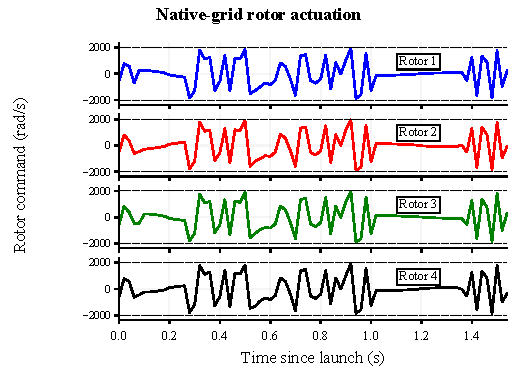
\includegraphics[width=\linewidth]{figures/team_execution.pdf}
\caption{Four signed rotor commands on a shared time axis. Separate panels expose each rotor's response; dashed lines mark the selected $\pm2000$ rad/s limit on the native 20 ms physics grid.}
\label{fig:teamexecution}
\end{minipage}\hfill
\begin{minipage}[t]{0.49\textwidth}\vspace{0pt}\centering
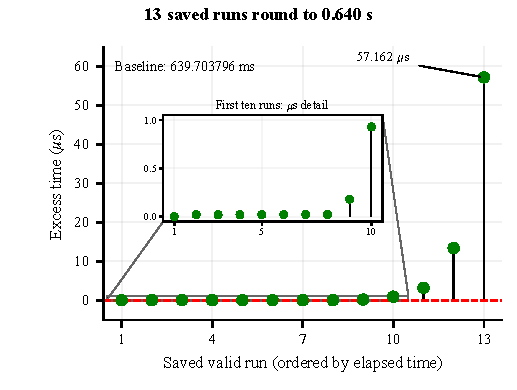
\includegraphics[width=\linewidth]{figures/team_repeatability_vector.pdf}
\caption{Variation among thirteen saved valid runs, ordered by elapsed time. Excess time is relative to 639.703796 ms. The inset resolves the tightly grouped first ten runs; the full view retains all thirteen.}
\label{fig:teamrepeatability}
\end{minipage}
\end{figure*}
\subsection{Course Implementation and Racing Extension}
The course pipeline initializes from the measured pose, plans position and unwrapped yaw through the gate poses, and publishes synchronized desired states.
Table~\ref{tab:deliverables} lists the four requested code components.
The fastest saved team run uses the separate discrete rigid-body optimizer and synchronous controller described below.
Both implementations use \texttt{/current\_state} and \texttt{/desired\_state}; the racing record also contains native Unity metadata and motor commands.
\begin{table}[!ht]\centering\small
\caption{Implementation of the requested LAB4 code components.}
\label{tab:deliverables}
\renewcommand{\arraystretch}{1.12}
\begin{tabularx}{\columnwidth}{lY}\toprule
Part&Implemented behavior\\\midrule
0&First-gate target with zero desired velocity and acceleration; desired-pose transform.\\
1.1&Current position and yaw initialized from odometry.\\
1.2&Position and continuous yaw vertices, shared segment times, and endpoint derivative constraints.\\
1.3&Time-aligned position, velocity, acceleration, and yaw sampled and published to the controller.\\\bottomrule
\end{tabularx}
\end{table}

\subsection{Discrete Rigid-Body Optimization}
We solve the racing reference on the native $h=0.02$ s physics grid.
The state contains position $\bm p$, velocity $\bm v$, rotation $R$, and world angular velocity $\bm\omega$; the inputs are four signed rotor thrusts $\bm f$.
Let $B$ map rotor thrusts to the wrench, with $F=(B\bm f)_1$ and $\bm\tau=(B\bm f)_{2:4}$.
The simulator-matched update is
\begin{align}
\bm v_{n+1}&=\bm v_n+h(F_nR_n\bm e_3/m-g\bm e_3),\\
\bm p_{n+1}&=\bm p_n+h\bm v_{n+1},\\
\bm\omega_{n+1}&=\bm\omega_n+hR_nJ^{-1}\bm\tau_n,\\
R_{n+1}&=\exp(h[\bm\omega_{n+1}]_\times)R_n.
\end{align}
The vehicle parameters are $m=1$ kg, $g=9.81$ m/s$^2$, arm length 0.3 m, $J=\operatorname{diag}(0.1,0.2,0.1)$ kg\,m$^2$, thrust coefficient $c_f=10^{-3}$, and drag coefficient $c_d=10^{-5}$.
The saved schedule allocates 0.300 s to launch, 0.640 s to racing, and 0.600 s to braking.
With normalized inputs $\bm u_n=\bm f_n/(c_f\Omega_{\max}^2)$, the fixed-schedule objective is
\begin{align}
J_{\rm rigid}={}&\sum_n\left[0.05\norm{\bm p_n-\bar{\bm p}_n}^2
+0.001\norm{\bm u_n}^2\right]\nonumber\\
&+0.003\sum_{n\geq1}\norm{\bm u_n-\bm u_{n-1}}^2.
\end{align}
Here $\bar{\bm p}$ is an initial interpolating curve, and the input-difference term starts at $n=1$.
The dynamics and input bounds $|u_{n,j}|\leq1$ are imposed as constraints.
Angular speed is limited to 6.85 rad/s and altitude to 0.65 through 5.1 m.
The trajectory must cross the gates forward in order and end at rest.
Horizontal and vertical offsets at scheduled crossings lie within $\pm0.15$ m.
Between gates, positions stay within a horizontal corridor of radius 2 m around the adjacent gate connections.

\subsection{Synchronous Feedforward and Feedback}
The controller reads one native Unity pose per physics step.
It estimates translational velocity by backward differences and angular velocity from the relative rotation of consecutive poses.
Reference acceleration and state feedback determine the translational command:
\begin{equation}
\bm F_c=m\left[\bm a_d+g\bm e_3+\gamma k_p(\bm p_d-\bm p)
+\gamma k_v(\bm v_d-\bm v)\right].
\end{equation}
The gains are $k_p=40$, $k_v=12$, and $\gamma=0.3$.
The attitude loop follows the reference rotation with a rotation-vector error gain of 12 and an angular-rate gain of 50.
Allocated rotor thrusts are clipped and converted using $\Omega_j=\operatorname{sgn}(f_j)\sqrt{|f_j|/c_f}$, with $|\Omega_j|\leq2000$ rad/s.
The simulator accepts signed commands.
Disabling rendering interpolation aligns pose reading and control with the physics grid while retaining the vehicle, gate, collision, and physics-step settings.
Each command is applied before the next native step.

\subsection{Timing and Evaluation Protocol}
We measure simulation time from the forward crossing of gate 1 to the forward crossing of gate 12.
For gate centre $\bm g_i$ and normal $\bm n_i$, a crossing requires a negative-to-positive change in $\bm n_i^\mathsf T(\bm p-\bm g_i)$.
Cubic Hermite interpolation of adjacent native positions and finite-difference velocities estimates the crossing time within its 20 ms bracket.
Horizontal and vertical offsets must both lie in $[-0.5,0.5]$ m.
The point-to-aperture-edge margin is
\begin{equation}
\mu_i=0.5-\max(|\eta_{h,i}|,|\eta_{v,i}|).
\end{equation}
The margin measures clearance of the interpolated crossing point, while collision messages record vehicle contact.
Preparation at the spawn position precedes trajectory launch.
All five initial floor contacts occur before launch; no collision is recorded during racing or braking.

We evaluate tracking error at native state timestamps against linear interpolation of the saved position reference.
The complete 1.54 s execution window contains 78 samples, and 31 native samples fall strictly within the interpolated gate-to-gate interval.
Table~\ref{tab:teamresult} reports both windows.

\subsection{Flight Results}
The best saved run passes all twelve gates in 639.703796 ms, displayed as 0.640 s, and reaches gate 12 in 939.843382 ms from launch.
Gate 12 has the smallest point margin, 0.287 m; gate 5 has the largest, 0.453 m.
Figure~\ref{fig:teamtracking} shows the measured course, tracking error, and aperture offsets.
Timed position RMSE is 0.06267 m and maximum error is 0.08868 m.
Across launch, racing, and braking, these values are 0.07120 and 0.09953 m.

\begin{table}[!ht]\centering\small
\caption{Measured team result. All durations use simulation time.}
\label{tab:teamresult}
\renewcommand{\arraystretch}{1.09}
\begin{tabularx}{\columnwidth}{Yl}\toprule
Metric&Value\\\midrule
Gate 1 to gate 12&\textbf{0.639704 s}\\
Launch to gate 12&0.939843 s\\
Ordered gates accepted&\textbf{12/12}\\
Minimum point aperture margin&0.28701 m\\
Timed RMSE / maximum error&0.06267 / 0.08868 m\\
Execution RMSE / maximum error&0.07120 / 0.09953 m\\
Racing and braking collisions&0\\
Peak / limit rotor command&1948.38 / 2000 rad/s\\
Peak native-pose speed&435.34 m/s\\
Saved valid 0.640 s runs&13\\\bottomrule
\end{tabularx}
\end{table}

Figure~\ref{fig:teamtracking}(c) plots native-pose speed, and Fig.~\ref{fig:teamexecution} shows signed rotor commands.
The peak command is 1948.38 rad/s, below the 2000 rad/s limit.
The 435.34 m/s peak speed is specific to this discrete simulator and signed-thrust configuration.
One 20 ms step at that speed spans approximately 8.71 m.
Gate-passage assessment uses crossing interpolation together with the simulator's contact record.

The original Unity XML and all 458 published state messages contain matching stored positions.
Recomputed crossings give 639.703797 ms with Hermite interpolation and 639.746866 ms with linear interpolation, both rounding to 0.640 s.
Figure~\ref{fig:teamframes} shows native frames immediately after the detected crossings, with interpolated event times in the panel titles and native-step times on the HUD.
The submission includes a flight video and the complete rosbag.

Thirteen saved valid runs round to 0.640 s.
Their elapsed times span 639.703796--639.760958 ms, a range of 57.162~$\mu$s.
Figure~\ref{fig:teamrepeatability} plots excess time relative to the best saved run.
Each point is one retained valid run.

\section{Team Roles and Core Personal Contributions}
\begin{table}[!ht]\centering\small
\caption{Team work allocation.}
\label{tab:teamallocation}
\renewcommand{\arraystretch}{1.12}
\setlength{\tabcolsep}{4pt}
\begin{tabularx}{\columnwidth}{@{}lYr@{}}\toprule
Member&Responsibilities&Share\\\midrule
Li Shuyu&Core trajectory planning and optimization; entry, racing, braking, and feasibility constraints.&20\%\\
Deng Chengyang&Feedback gains, rotor allocation, position errors, and rotor limits.&20\%\\
Zhou Jingxin&Unity/ROS integration, synchronous stepping, and state alignment.&20\%\\
Zhou Chunyang&Ordered gate timing, bag replay, and contact checks.&20\%\\
Zhang Yuxin&Video alignment, figures, and repeated-run summaries.&20\%\\\bottomrule
\end{tabularx}
\end{table}

My trajectory formulation and optimized reference provided the core planning basis of the team's reported 0.640 s result.
I determined the scheduled gate crossings and the state and rotor-thrust sequence connecting entry, racing, and braking.
This work resolved the central planning task: turning the selected race timing into a complete motion that satisfied the imposed geometric, dynamic, and terminal constraints.
The synchronous controller executed this reference in the measured twelve-gate run.

\subsection{Mathematical Foundation of Trajectory Planning}
I established the mathematical basis of the individual planning work by deriving the single-segment quadratic programs, including the terminal-velocity constraint, and obtaining their polynomial solutions.
I then formulated the multi-segment minimum-snap problem, counted the endpoint and continuity conditions, and derived the natural conditions at intermediate waypoints.
These derivations specify the degrees of freedom and boundary conditions that determine the optimized motion.

In the single-segment analysis, I connected the quadratic objective to a global lower bound and examined how an additional endpoint velocity changes the solution.
For minimum snap, I distinguished the conditions imposed on each segment from the conditions produced by optimality at a shared waypoint.
This distinction accounts for continuity of derivatives four through six when the internal lower-order derivatives are free.
I used the resulting condition count to explain the polynomial degree and the structure of the multi-segment system.

\subsection{Experimental Basis for Timing Selection}
I designed and implemented the numerical comparisons used to explain the relationship between trajectory timing and trackability.
I compared stopping and global references at matched durations.
My analysis covered time scaling, acceleration lag, saturation, and the response-time sweep.
I used position RMSE, maximum error, snap cost, and the saturated-sample fraction to relate tracking performance to reference demand.
The matched ablations separated the effects of lag and saturation, and the step-size comparison assessed numerical sensitivity.
Together, these experiments explained why a shorter reference can increase tracking error even when its spatial path remains unchanged.

I kept the course, initial state, feedback gains, and model parameters fixed within each matched comparison.
For time scaling, I related the numerical trends to the derivative scaling laws and the $\alpha^{-7}$ dependence of integrated snap.
For the response-time sweep, I identified the shortest tested duration satisfying the stated maximum-error threshold at each lag.
I also derived the lag-only error equation and its stability condition, connecting reference jerk to tracking error and giving the ablation results a dynamical interpretation.

\subsection{Core Racing-Trajectory Design}
I took primary responsibility for the team's trajectory optimization, which determined the planned motion over the complete flight.
I formulated the reference on the native 20 ms physics grid with position, velocity, attitude, angular velocity, and four rotor-thrust inputs.
The saved schedule assigns 0.300 s to entry, 0.640 s to racing, and 0.600 s to braking.
Optimizing these phases together connects the scored gate crossings to a dynamically constrained entry and a zero-velocity stopping state.

I expressed the coupled state and input optimization in CasADi and used IPOPT to solve it.
The formulation carries translational motion, rotation, and angular velocity through the same sequence of physics steps.
An interpolating curve through the starting point, gate centres, and stopping point defines the path-deviation penalty.
I normalized the rotor inputs by the thrust associated with the selected rotor-speed limit, so each input bound has a consistent scale.
The input-effort and input-difference terms balance the path penalty against the magnitude and variation of the required thrusts.

\subsection{Dynamic Feasibility and Executable Reference}
I made geometric and dynamic feasibility part of the trajectory design by imposing forward gate-plane crossings and bounding the horizontal and vertical offsets at each scheduled passage.
Altitude, angular-speed, rotor-thrust, and inter-gate corridor constraints restricted the motion between gates.
The zero terminal-velocity condition defined the braking endpoint.

At each scheduled gate, I required the vehicle to lie on the gate plane with positive normal velocity.
Neighbouring trajectory nodes remain on opposite sides of that plane, which encodes the direction of passage across consecutive steps.
The optimized horizontal and vertical offsets are restricted to $\pm0.15$ m inside the $\pm0.5$ m aperture.
Between gates, the corridor constraint bounds horizontal deviation from the adjacent gate connection.
These constraints determine where and in which direction the optimized motion passes each gate.
Including a braking segment also requires the fast passage trajectory to connect to a zero-velocity endpoint within the same state and input model.

I produced the complete reference used by the synchronous controller, with optimized position, velocity, acceleration, attitude, angular velocity, and rotor thrusts on a common timeline.
The controller used this reference for feedforward thrust commands and feedback tracking.
Executing it with the team's feedback, simulator integration, and timing components yielded the twelve-gate result of 0.639704 s with 0.06267 m timed position RMSE in Table~\ref{tab:teamresult}.
My work provided the essential planning basis for that result by turning the course geometry and race schedule into a dynamically constrained flight from entry to braking.

\section{Discussion and Conclusion}
Polynomial degree controls trajectory shape freedom, internal derivative constraints control motion through waypoints, and duration sets the controller's motion demand.
Higher degree helps when added constraints restrict the lowest-degree solution.
Freeing internal derivatives reduces repeated acceleration and braking, while time compression increases derivative magnitudes on the same spatial curve.

On the numerical course, global minimum snap reduces the objective by 98.98\% at the same duration as the stopping reference.
Compressing it to 8.4 s produces frequent acceleration saturation and meter-scale position errors.
Saturation has the larger isolated-model error at the most aggressive timing, while lag raises corrective acceleration demand.
Timing should be reduced from a well-tracked reference while monitoring position error, saturation, and gate clearance.
Unequal segment times can give sharp turns more time than long straight sections.

The team reference completes the twelve-gate interval in 0.640 s of simulation time with 0.06267 m timed position RMSE and 0.287 m minimum point aperture margin.
Native-state recomputation and thirteen saved valid runs support this timing measurement.
The individual experiments quantify smoothness and response limits, and the team experiment records execution in the specified simulator.
These results support selecting race timing from measured tracking error and gate clearance under the intended controller settings.
\begin{thebibliography}{9}
\bibitem{mit} MIT VNAV, ``Lab 4: Exercises,'' 2023. [Online]. Available: \url{https://vnav.mit.edu/labs_2023/lab4/exercises.html}. Accessed: Nov. 9, 2026.
\bibitem{code} MIT-SPARK, ``VNAV-labs, release VNAV2021.'' [Online]. Available: \url{https://github.com/MIT-SPARK/VNAV-labs/releases/tag/VNAV2021}. Accessed: Nov. 9, 2026.
\bibitem{library} ETH Zurich Autonomous Systems Lab, ``mav\_trajectory\_generation: Polynomial trajectory generation and optimization.'' [Online]. Available: \url{https://github.com/ethz-asl/mav_trajectory_generation}. Accessed: Nov. 9, 2026.
\end{thebibliography}
\end{document}
